\documentclass[tikz, border=10pt]{standalone}
\usetikzlibrary{positioning, arrows.meta}

\begin{document}
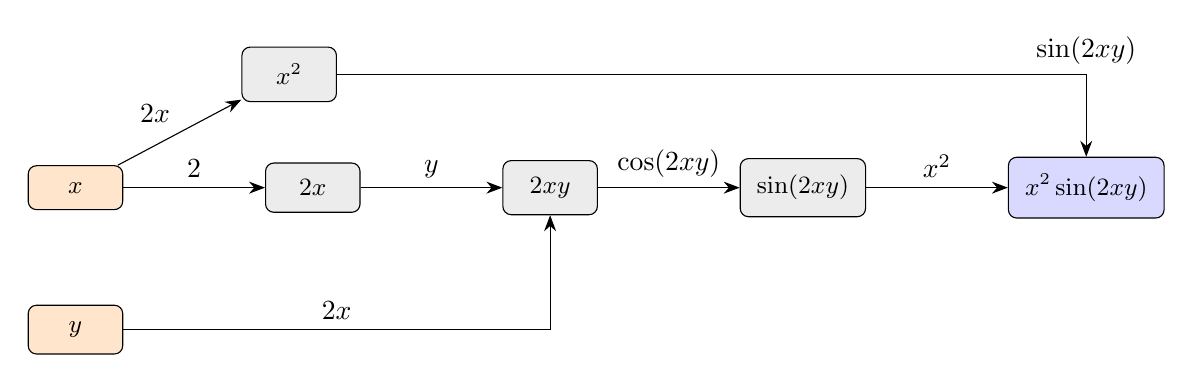
\begin{tikzpicture}[
    % Set global spacing
    node distance=1.2cm and 1.8cm,
    % Define box styles
    base/.style={draw, rounded corners=3pt, inner sep=6pt, minimum width=1.2cm, font=\small},
    input/.style={base, fill=orange!20},
    op/.style={base, fill=gray!15},
    output/.style={base, fill=blue!15},
    % Arrow style
    >={Stealth[scale=1.2]}
]

    % --- NODES ---
    \node[input]  (x) {$x$};
    \node[input, below=of x] (y) {$y$};

    % Operations
    \node[op, above right=0.8cm and 1.5cm of x] (x2) {$x^2$};
    \node[op, right=of x] (2x) {$2x$};
    \node[op, right=of 2x] (2xy) {$2xy$};
    \node[op, right=of 2xy] (sin) {$\sin(2xy)$};
    
    % Final Output
    \node[output, right=of sin] (final) {$x^2 \sin(2xy)$};

    % --- EDGES ---
    % Path from x to x^2
    \draw[->] (x) -- node[midway, above left] {$2x$} (x2);
    
    % Path from x through middle
    \draw[->] (x) -- node[midway, above] {$2$} (2x);
    \draw[->] (2x) -- node[midway, above] {$y$} (2xy);
    
    % Path from y to 2xy (using a bent arrow)
    \draw[->] (y) -| node[pos=0.25, above] {$2x$} (2xy);
    
    % Continue through sin
    \draw[->] (2xy) -- node[midway, above] {$\cos(2xy)$} (sin);
    \draw[->] (sin) -- node[midway, above] {$x^2$} (final);
    
    % Top path from x^2 to final
    \draw[->] (x2) -| node[pos=0.5, above] {$\sin(2xy)$} (final);

\end{tikzpicture}
\end{document}